\documentclass{report}
\usepackage{amsmath,caption,float,geometry,titlesec,tikz,tkz-euclide,amssymb}

\begin{document}

\title{Projective Geometery}
\author{Ruchith R}
\date{}

\section*{Reference Formuale}
Focus : $(ae,0)$

\noindent Directrix : $x = \frac{a}{e}$
\subsection*{Parabola $(e = 1)$}

Equation : $$y^2 = 4ax$$

\noindent Parametric form : $(at^2,2at)$

\subsection*{Ellipse $(0 < e < 1)$}
Equation : $$\frac{x^2}{a^2} + \frac{y^2}{b^2} = 1$$

\noindent Parametric form : $(a\cos t,b\sin t)$

\subsection*{Hyperbola $(e > 1)$}
Equation : $$\frac{x^2}{a^2} - \frac{y^2}{b^2} = 1$$

\noindent Parametric form : $(a\sec t,b\tan t)$

\section*{Group law on Parabola}

Given any parabola, there exists an affine transformation that takes it to the curve $y = x^2$.
\begin{figure}[H]
    \centering
    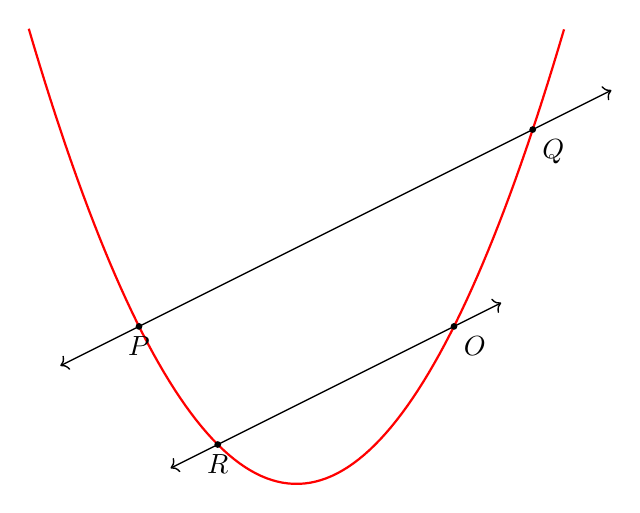
\begin{tikzpicture}[scale=2]
        \draw[thick,red,domain=-1.7:1.7,samples=100] plot (\x,{(\x)^2});
        \tkzDefPoint(1,1){O}
        \tkzDefPoint(-0.5,0.25){R}
        \tkzDefPoint(-1,1){P}
        \tkzDefPoint(1.5,2.25){Q}
        
        \tkzDrawLine[<->,line width=0.5,add=0.2 and 0.2](P,Q)
        \tkzDrawLine[<->,line width=0.5,add=0.2 and 0.2](O,R)
        
        \tkzDrawPoints[fill=black](O,P,Q,R)
        \tkzLabelPoints[below right](O)
        \tkzLabelPoints[below](P)
        \tkzLabelPoints[below right](Q)
        \tkzLabelPoints[below](R)
    \end{tikzpicture}
    \caption{$R = P\oplus Q$}
\end{figure}

We define the parametric coordinates of the point $R$ as $(r,r^2)$.
We compare the slopes of the two lines $PQ$ and $OR$ to obtain the co-ordinates of $R$.
\[\frac{r^2-o^2}{r-o} = \frac{p^2-q^2}{p-q}\]
\[r = p+q-o\]
We define a homomorphism from the points on the parabola to R as $\phi((x,x^2)) = x-o$.
The map that is defined is a bijection hence it is an isomorphism.
The curve shown in the figure is $\mathbb{R}^2$ however the algebra performed remains the same if the field is changed to $\mathbb{C}^2$ .

\section*{Solving for curves in finite fields}

We first investigate the solution set of a curve when working with finite field $\mathbb{Z}_p$.
\[\mathcal{C}  = \{(x_1,x_2,\cdots,x_n) \in \mathbb{Z}_p^n \text{ }|\text{ } condition \} \subseteq \mathbb{Z}_p^n\]
We notice that $\mathbb{Z}_p^n$ contains a finite number of points ($p^n$) and so will $V$.
So it is a valid approach to just verify which points out of these will satisfy the condition.
\vspace{1ex}

\noindent We now see the solution for one such problem
\[V = \{(x,y,z) \in \mathbb{Z}_p^3 \text{ }| x^2+y^2 = z^2\}\]
We take a different approach to the problem.
We set $z$ as a parameter and plot the various curves for different values of $z$.
Now the problem is simplified to two variables for each value of $z$.
We see that we can embed $\mathbb{Z}_p^2 \text{ in } \mathbb{R}^2$ such that $\mathbb{Z}_p^2 \subset \mathbb{R}^2$.

For every $z \in \mathbb{Z}_p$, 
Define $\mathcal{V}_z = \{(x,y) \text{ }| x^2+y^2=z^2\}$

Notice that: 
\[V = \bigcup_{z \in \mathbb{Z}_p}\mathcal{V}_z\cap\mathbb{Z}_p^2 \]
\begin{figure}[H]
    \centering
    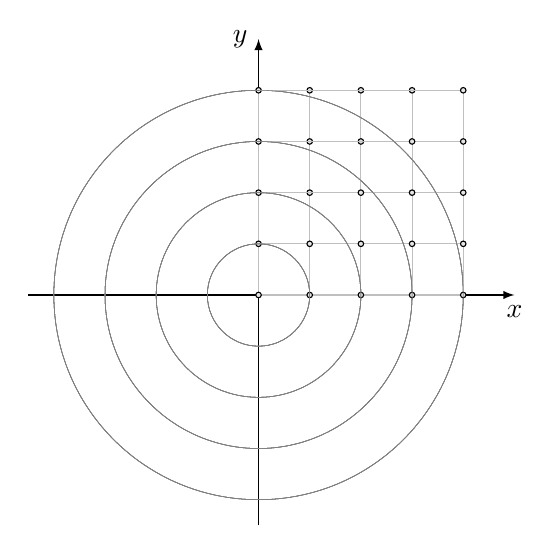
\begin{tikzpicture}[scale=0.65]
        \tkzInit[xmin=-4.5,xmax=4.5,ymin=-4.5,ymax=4.5]
        \tkzDrawX
        \tkzDrawY
        \foreach \x in {0,...,4} {
            \draw[gray!50] (\x,0) -- (\x,4);
            \draw[gray!50] (0,\x) -- (4,\x);
            \foreach \y in {0,...,4} {
                \tkzDefPoint(\x,\y){P\x\y}
                \tkzDrawPoint(P\x\y)
            }
            \tkzDefPoints{0/0/A,1/0/a,2/0/b,3/0/c,4/0/d}
            \tkzDrawCircles(A,a A,b A,c A,d)
          }
    \end{tikzpicture}
    \caption{The figure represents the $mod$ 5 solutions}
\end{figure}

\end{document}